\chapter{Motivating Scenario}
\label{chap:motivatingScenario}
In order to help in understanding the concepts of organizational modeling, a motivating scenario has been taken and explained through the notations mentioned in Chapter \ref{chap:fundamentals}. This scenario also helps in validating the developed web editor in the following Chapter \ref{chap:casestudy}. The motivating scenario has been chosen based on the collected real life scenarios provided in the thesis work of the author Sierra\cite{Sierr2015}. The motivating scenario was taken from the context of manufacturing sector. 

In this chapter, the first section provides a brief introduction about the motivating scenario. The last section provides an abstract overview about the entity types discussed in motivating scenario. This abstract concepts are explained in a concrete way in the following Chapter \ref{chap:casestudy}.

%%%%%%%%%%%%%%%%%%%%%%%%%%%%%%%%%%%%%%%%%%%%%%%%%%%%%%%%%%%%%%%%%%%%%%%%%
\section{Resource-centric Organizational Modeling Example}
\label{sec:scenario}
%%%%%%%%%%%%%%%%%%%%%%%%%%%%%%%%%%%%%%%%%%%%%%%%%%%%%%%%%%%%%%%%%%%%%%%%%
 The concept of resource centric organizational modeling can be explained with the following scenario taken from a manufacturing organization. Consider, a budding manufacturing company which designs, develops, manufactures and sells personal computers, tablets and laptops. The CEO's main intention of the quarter is \textit{to increase the revenue and number of unit sales}. The initial context describes the situation before starting the execution of intention. The initial context also provides description that motivates to start the process. The final context describes the situation that is achieved once the intention executed successfully. Intentions connect initial context definitions with final context definitions \cite{Sungur2014a}. The sub-intentions are the intermediate intentions which describes the expected outcome in a measurable form. Intentions reach strategy implementations through achieving strategies which are plans of action designed to meet a specific intention. 
 
  \begin{figure}
  	\centering
  	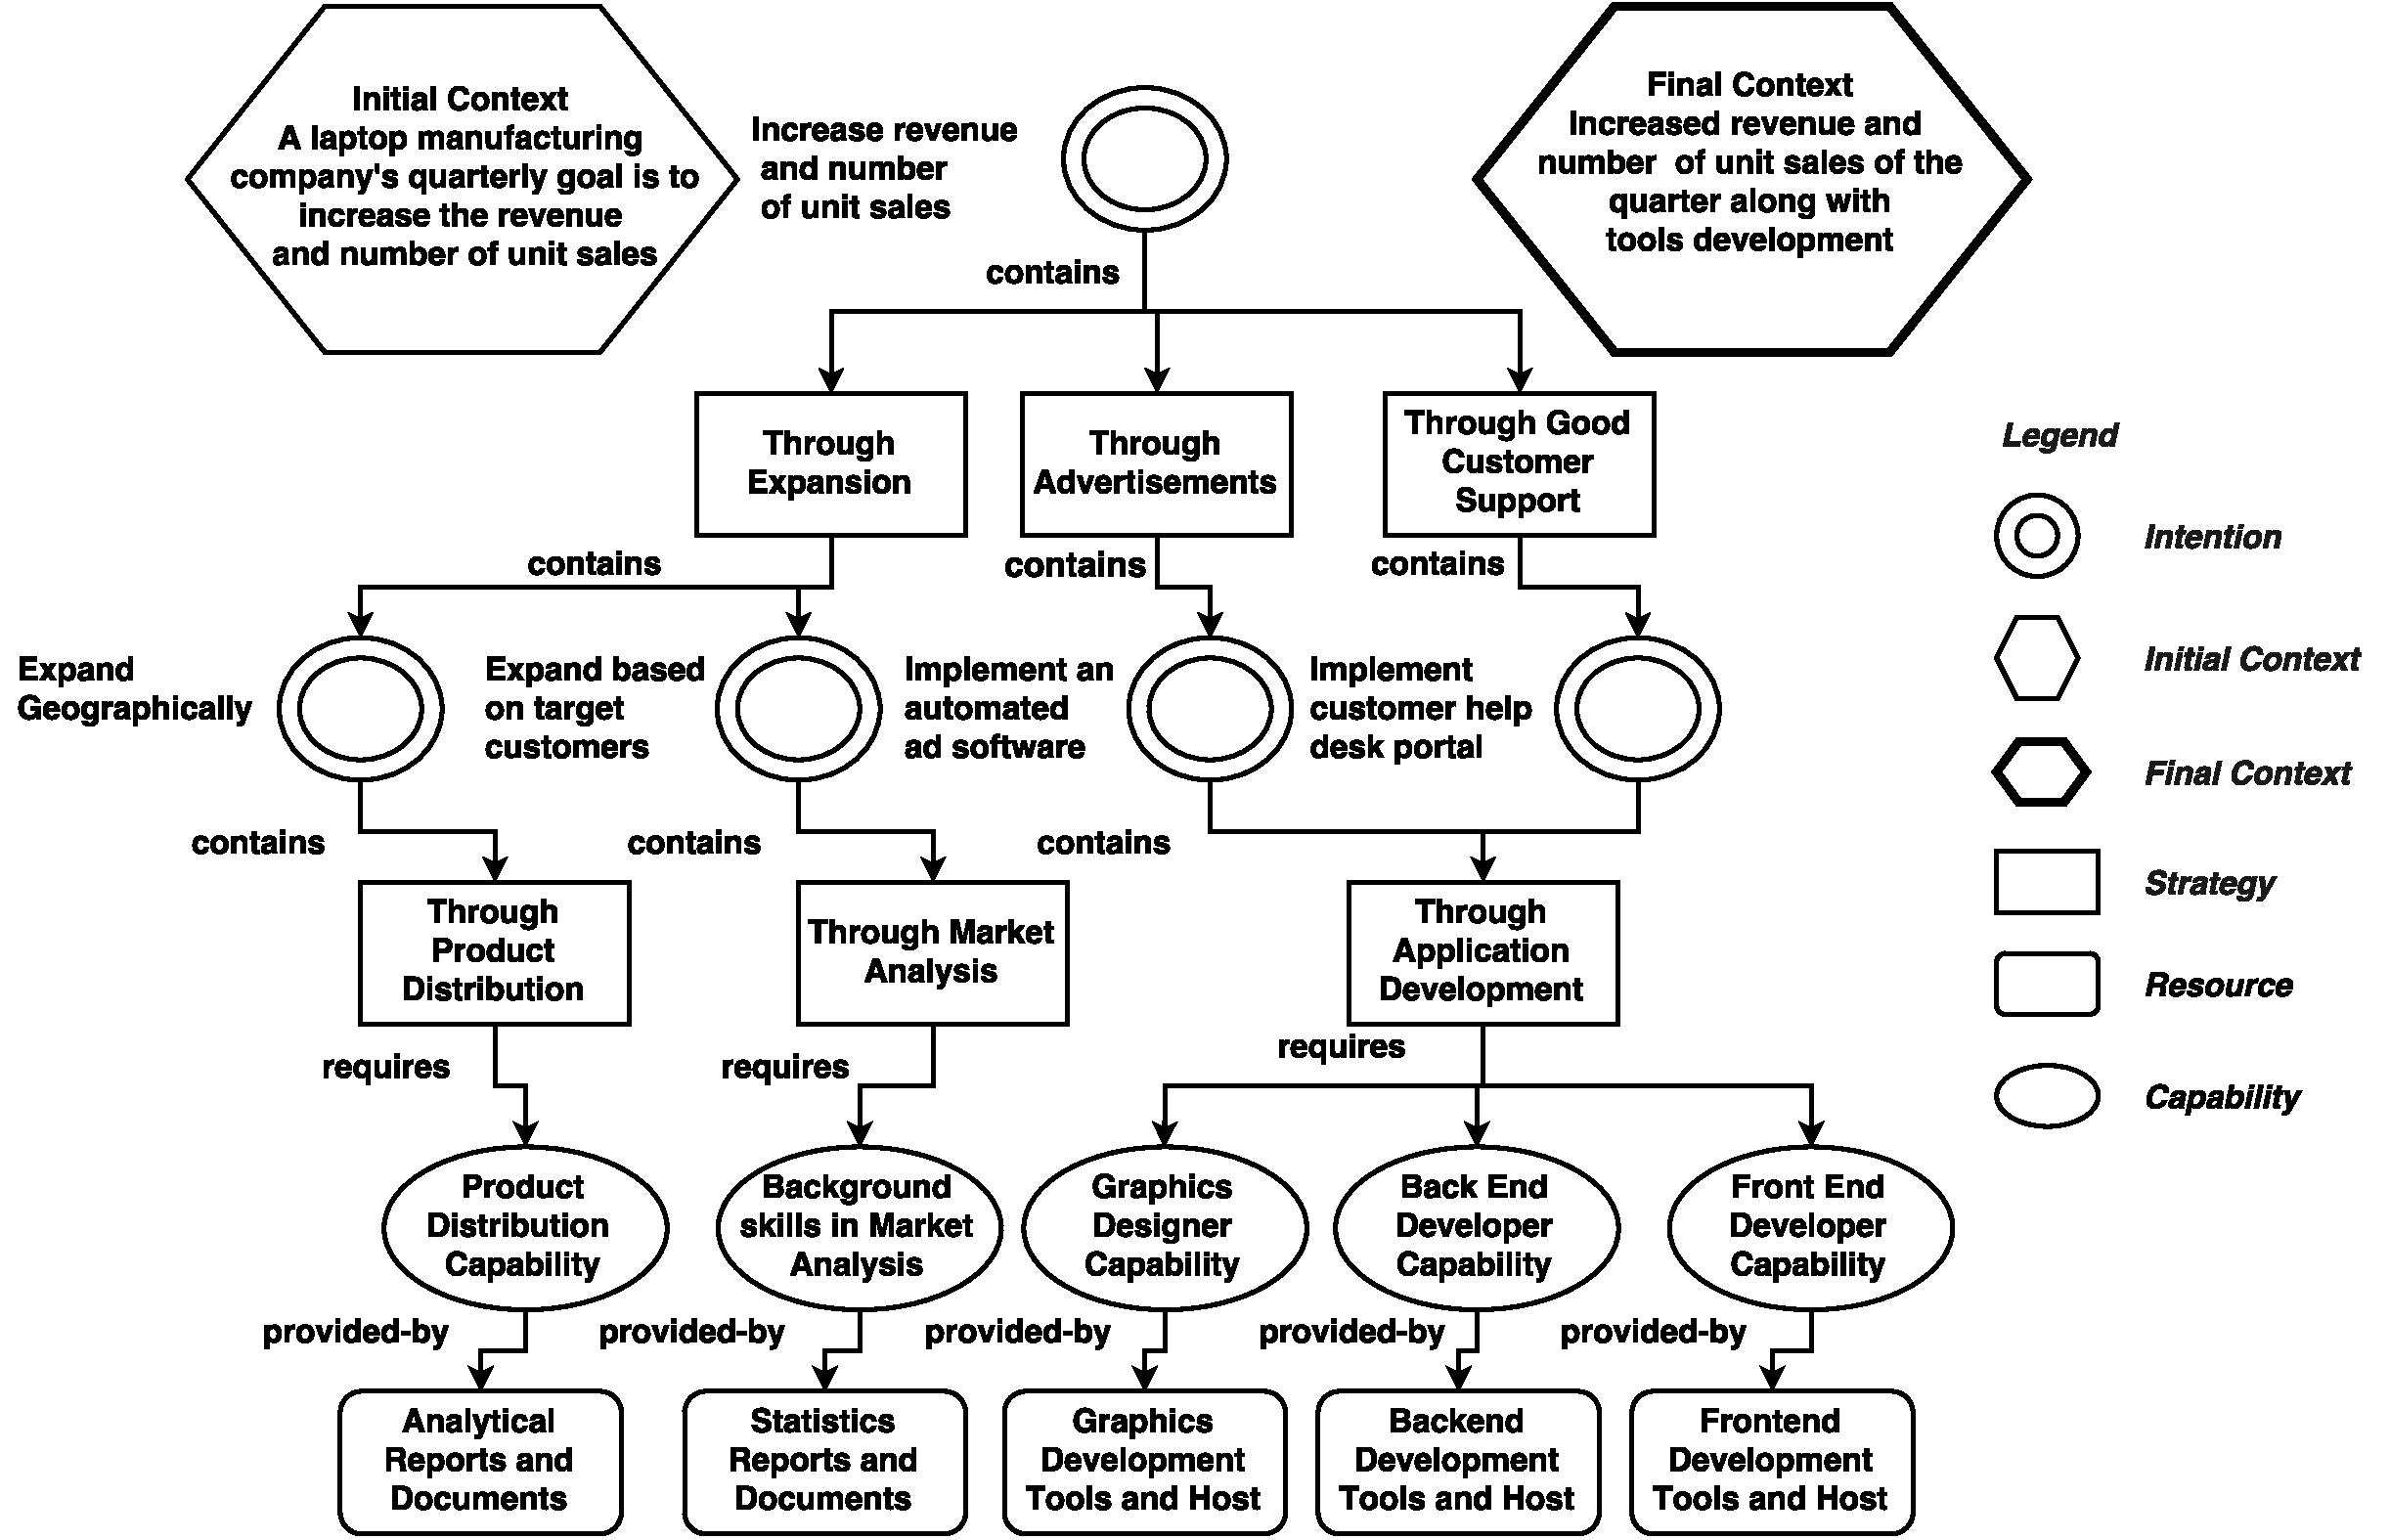
\includegraphics[width=\textwidth,angle=0]{MotivatingScenario.pdf}
  	\caption{Motivating Scenario}
  	\label{fig:motivatingscenario}
  \end{figure}
  
The example scenario follows a top-down approach of organizational modeling i.e., higher abstract level intentions can be achieved by amalgamation of specific, measurable and realistic sub-intentions, strategies etc. The figure\ref{fig:motivatingscenario} provides the details of intention and its associated strategies, sub-intentions. There can be multiple strategies followed to achieve an intention. In this type of process modeling, strategies are self-contained and loosely coupled  \cite{Sungur2014a}. This is the reason when we extract only the strategies from organizational process modeling it would realize the informal process essential models. 
 
In order to achieve this main intention through our resource-centric modeling approach, first we need to break the intention into concrete levels like strategies, sub-intentions, process definitions, resource definitions etc. This intention can be achieved by following all of the below mentioned strategies and sub-intentions, which requires resources with matching capabilities associated with strategies. 
 
 \begin{enumerate}
 	\item Increasing the revenue through expanding the market sales. 
 	\item Through increasing the advertisement which helps in customer to know about the product.
 	\item Improving the existing customer help desk portal, as it helps to maintain good customer relationship.
 \end{enumerate}
 
%%%%%%%%%%%%%%%%%%%%%%%%%%%%%%%%%%%%%%%%%%%%%%%%%%%%%%%%%%%%%%%%%%%%%%%%%
\section{An Abstract View of Entity Types}
\label{sec:entities}
%%%%%%%%%%%%%%%%%%%%%%%%%%%%%%%%%%%%%%%%%%%%%%%%%%%%%%%%%%%%%%%%%%%%%%%%%
This section discusses in details, about each entity types of the motivating scenario in an abstract way, which is further detailed using concrete steps in the following Chapter \ref{chap:casestudy}. The participating resources work towards one \textit{main intention} and certain \textit{sub-intentions}. Sub-intentions are part of main intention, which helps the resources to modularize and achieve the main intention. Also each sub-intention has certain type of relationship with main-intention. For example in our below described motivating scenario in Section \ref{sec:scenario} one of the sub-intention is to \textit{expand sales geographically}. Before executing this sub-intention, few ground works like collection of laptop usage statistics such as average buying capacity of the consumers, average computer knowledge in the new area has to be done. Thus the execution of main intention i.e \textit{increase revenue and number of unit sales}, requires collaboration of people with different skills and expertise. People with skills to collect and study statistics can serve as external resources. As new intentions may emerge dynamically, the team working towards the achievement of main intention should also be ready to accommodate new resources with new capabilities and skills. For example, there is a software development team, which work towards achievement of one of the sub-intention \textit{improve help desk portal}, i.e this team develops software that automatically attends and records user queries. Suppose, if there arise a new requirement of \textit{supporting help desk thorugh mobile applications} as well then the system should accommodate new resource with \textit{mobile application developer} capability. The management of this project resource is considered to be done through the support of project management software called Redmine \footnote{http://www.redmine.org/}. The participating human resources are members of business oriented social network called XING \footnote{http://www.xing.com/}.

%%%%%%%%%%%%%%%%%%%%%%%%%%%%%%%%%%%%%%%%%%%%%%%%%%%%%%%%%%%%%%%%%%%%%%%%%
\subsection{Contexts} 
\label{sec:contexts}
%%%%%%%%%%%%%%%%%%%%%%%%%%%%%%%%%%%%%%%%%%%%%%%%%%%%%%%%%%%%%%%%%%%%%%%%%
The execution of manufacturing processes such as the one provided in Figure \ref{fig:motivatingscenario}, are not similar to execution of typical business processes. This is because, the execution of manufacturing processes mostly depends on the information collected from the real world, i.e., the execution context \cite{Sungur2016}. A context definition provides mechanism to act adaptively based on the current situation. This is achieved in the production environment by describing each process with a specific context definition \cite{Sungur2016}. For example, in our motivating scenario the initial context provides details about status before achievement of the main intention i.e it specifies the situation of the organization which triggers the execution of main-intention. The initial context \textit{quarterly goal of increasing the revenue and number of unit sales}, helps to decide the main intention and its related low level associates. On successful achievement of main-intention the organization reaches it desired final context of \textit{increased revenue and number of unit sales}. Along with successful reaching of the final context, this also provides tools such as web-based help desk portals, automated ad software etc., that are developed as part of this execution. When one of the final context definitions has been reached the process completion starts. This process final state can be stored\footnote{C.Timurhan Sungur, An Approach to Supporting and Automating Informal Processes, May 2015.} and same set of resources can be re-used in future executions with similar contexts and intentions.
 
%%%%%%%%%%%%%%%%%%%%%%%%%%%%%%%%%%%%%%%%%%%%%%%%%%%%%%%%%%%%%%%%%%%%%%%%%
\subsection{Intentions} 
\label{sec:intentions}
%%%%%%%%%%%%%%%%%%%%%%%%%%%%%%%%%%%%%%%%%%%%%%%%%%%%%%%%%%%%%%%%%%%%%%%%%
Intentions are defined hierarchically, in our approach intentions are in top level of the hierarchy, which are refined until concrete lower level of the hierarchy is reached. In this thesis context, intentions are not associated with capabilities directly, instead intentions are associated with strategies which are then associated with capabilities. For example, in our motivating scenario the main intention is to increase revenue and number of unit sales which also has sub-intention of \textit{improving the customer help desk portal} and strategies such as 1. through expanding sales and 2. through advertisements. The relation between strategies and intentions are denoted by the term \textit{achieved-through} in Figure \ref{fig:motivatingscenario} as strategies are methods through which intentions can be achieved. The relation between an intention ans its sub-intentions are denoted as \textit{contains} as intentions can contain and contradict themselves. For example, in our motivating scenario there can be a situation where customer help desk team not willing to give up the systems they are working for a long time even if it is a better solution for organization as whole. This can also happen in every organizations, where a real life scenario has been provided in the thesis work \cite{Sierr2015} and also it has been suggested that such contradicting intentions has to be handled in some way. Thus our developed web editor has provision to associate both sub-intentions and contradicting intentions for any intention. There are also sub-intentions that emerge through strategies which are also denoted by the term \textit{contains}. For example, in our motivating scenario, one of the strategy to increase the revenue and number of unit sales is through expanding the sales which further has sub-intentions such as \textit{expand geographically} and \textit{expand based on target customers}. 

%%%%%%%%%%%%%%%%%%%%%%%%%%%%%%%%%%%%%%%%%%%%%%%%%%%%%%%%%%%%%%%%%%%%%%%%%
\subsection{Strategies} 
\label{sec:strategies}
%%%%%%%%%%%%%%%%%%%%%%%%%%%%%%%%%%%%%%%%%%%%%%%%%%%%%%%%%%%%%%%%%%%%%%%%%
Strategies are used to identify the most appropriate method of utilizing the capabilities through which an intention can be achieved. Strategies are associated with both intentions and capabilities. Capabilities are related to resources. Each strategy needs certain capability to successfully execute an intention. Resources are the potential holder of the capability i.e., to satisfy a capability we need resources. Capability and its associated resources are also shown in the Figure \ref{fig:motivatingscenario}. In our motivating scenario, the main intention can be achieved through two strategies \textit{through expansion} and \textit{through advertisements}. These two strategy further contains intentions such as \textit{expand geographically}, \textit{expand based on target customers} and \textit{implement an automated ad software}. Since strategies contain intentions they are related through the term \textit{contains} in the Figure \ref{fig:motivatingscenario}.

\begin{figure}
	\centering
	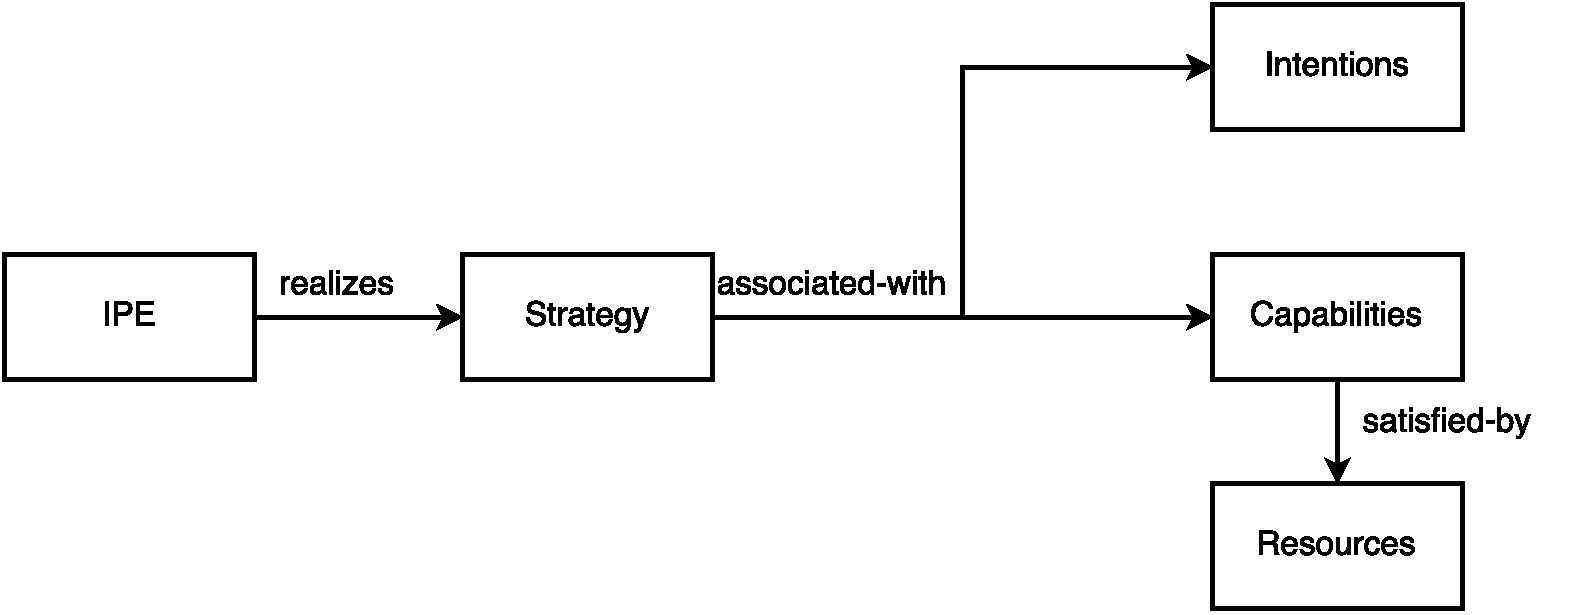
\includegraphics[width=\textwidth,angle=0]{SrtategiesasIPE.pdf}
	\caption{Relation of Strategy with IPE}
	\label{fig:strategiesasIPE}
\end{figure}


As mentioned before in the Chapter \ref{chap:fundamentals}, informal process models are realized through strategies. This is achieved through strategy containing capabilities and resources. For example, consider a small part in our motivating scenario of achieving an intention expand geographically through strategy product distribution. To acheive this intention through a specified strategy we need resources with product distribution capability. This results in informal process as a strategy that has capabilities, resources that are created out of capabilities and an intention of that specific strategy which is showed in the Figure \ref{fig:strategiesasIPE}.

%%%%%%%%%%%%%%%%%%%%%%%%%%%%%%%%%%%%%%%%%%%%%%%%%%%%%%%%%%%%%%%%%%%%%%%%%
\subsection{Capabilities}
\label{sec:capabilities}
%%%%%%%%%%%%%%%%%%%%%%%%%%%%%%%%%%%%%%%%%%%%%%%%%%%%%%%%%%%%%%%%%%%%%%%%%
Resources tends to posses certain capabilities that allow them to do something that they want or need to do something. Each organizational capability must be provided by a resource in the organization. Resource models are optional \footnote{C.Timurhan Sungur, An Approach to Supporting and Automating Informal Processes} to make precise definitions of resources needed. In our context, capabilities that are associated with resources are called as \textit{functional capabilities}. The type of capability that contains functional capabilities are called as \textit{cross functional capabilities}. Strategies are associated with cross functional capabilities, which contains functional capabilities out of which resources are created. In our motivating scenario to achieve the main intention, we need several capabilities such as product distribution capability, graphics designer capability etc. Thus in the Figure \ref{fig:motivatingscenario}, strategies and associated capabilities are related through the term \textit{satisfied-by}. 

%%%%%%%%%%%%%%%%%%%%%%%%%%%%%%%%%%%%%%%%%%%%%%%%%%%%%%%%%%%%%%%%%%%%%%%%%
\subsection{Resources} 
\label{sec:resources}
%%%%%%%%%%%%%%%%%%%%%%%%%%%%%%%%%%%%%%%%%%%%%%%%%%%%%%%%%%%%%%%%%%%%%%%%%
Each resources has different types of relationship with other resources based on how they communicate with other resources \cite{Sungur2015}. For example in our motivating scenario described in Section \ref{sec:scenario} has sub-intention of \textit{improve customer help desk portal}. This sub-intention can be achieved by providing skills improvement training to the employees or by recuriting newly skilled employee. Here the manager has permissions to decide whether to improve skills of existing employee or recruit new employee. But the team lead has restricted permission like what type of skills are required for the project based on decision of manager. The Informal Process Essentials (IPE) approach proposed by Sungur et al. \cite{Sungur2015}, paves the way to create models with definitions of key actors e.g manager, team lead and definitions of suppoting resources such as Mediawiki \footnote{http://www.mediawiki.org/}. A \textit{resource organizer} is responsible for gathering definitions about the resources which are required by business experts for modeling \cite{Sungur2014a}.  


